\documentclass[12pt, twoside]{article}
\usepackage[letterpaper, margin=1in, headsep=0.5in]{geometry}
\usepackage[english]{babel}
\usepackage[utf8]{inputenc}
\usepackage{amsmath}
\usepackage{amsfonts}
\usepackage{amssymb}
\usepackage{tikz}
\usetikzlibrary{quotes, angles}
\usepackage{graphicx}
\usepackage{enumitem}
\usepackage{multicol}
\usepackage{hyperref}

\newif\ifmeta
\metatrue %print standards and topics tags

\title{IB Mathematics}
\author{Chris Huson}
\date{February 2022}

\usepackage{fancyhdr}
\pagestyle{fancy}
\fancyhf{}
\renewcommand{\headrulewidth}{0pt} % disable the underline of the header
\raggedbottom


\fancyhead[LE]{\thepage}
\fancyhead[RO]{\thepage \\ Name: \hspace{4cm} \,\\}
\fancyhead[LO]{BECA / IB Math 4-Polynomial and rational functions \\* 9 February 2022}

\begin{document}

\subsubsection*{4.9 PreQuiz: Polynomial and rational functions}
\begin{enumerate}
\item The graph of a function $f$ is shown on the grid below.
    \begin{multicols}{2}
    \begin{enumerate}
      \item Write down $f(0)$
      \item Find $x$ for $f(x)=-3$.
      \vspace{0.25cm}
      \item Write down the domain.
      \item Write down the range. \vspace{1cm}
    \end{enumerate}
      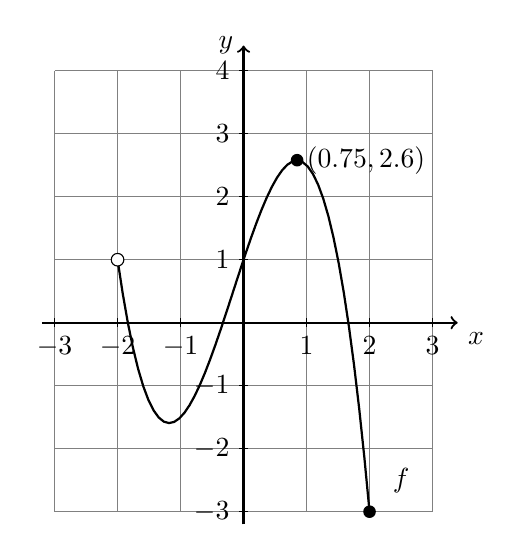
\begin{tikzpicture}[scale=0.8]
        \draw [help lines] (-3,-3) grid (3,4);
        \draw [thick, ->] (-3.2,0) -- (3.4,0) node [below right] {$x$};
        \draw [thick, ->] (0,-3.2)--(0,4.4) node [left] {$y$};
        \foreach \x in {-3,-2,-1,1,2, ...,3} \draw (\x cm,2pt)--(\x cm,-2pt) node[below] {$\x$};
        \foreach \y in {-3,-2,-1,1,2,3,4} \draw (2pt,\y cm)--(-2pt,\y cm) node[left] {$\y$};
        \draw [thick,samples=50,domain=-2:2] plot(\x,-\x^3-0.5*\x*\x+3*\x+1);
        \fill (2,-3) circle[radius=0.1];
        \fill (0.85,2.58) circle[radius=0.1] node [right]{$(0.75,2.6)$};
        \node at (2.5,-2.5){$f$};
        \fill [white] (-2,1) circle[radius=0.1];
        \draw (-2,1) circle[radius=0.1];
      \end{tikzpicture}
    \end{multicols}

\item Part of the function $f(x)=x^3-2x^2-5x+6$ is shown on the graph.
    \begin{center}
    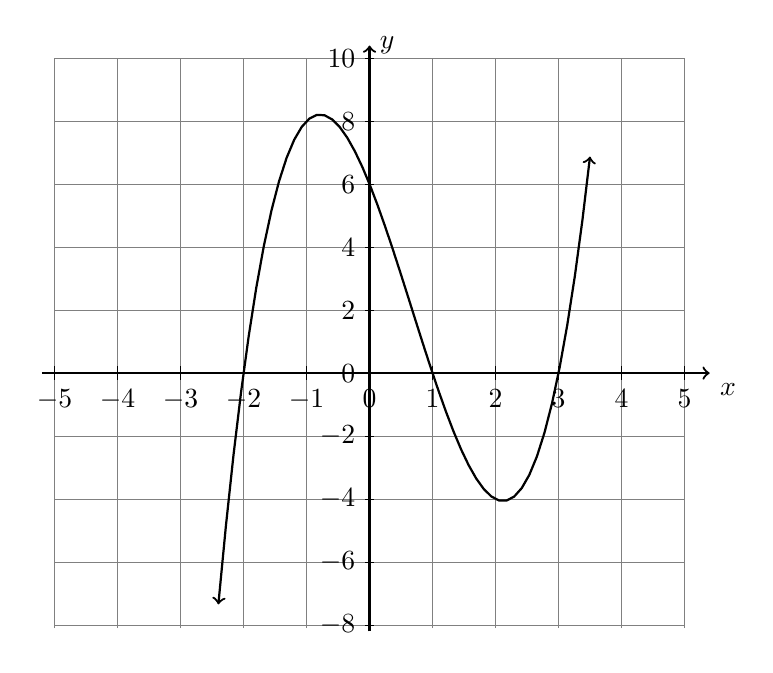
\begin{tikzpicture}[x=1cm, y=0.5cm, scale=0.8]
        \draw [help lines] (-5,-8.1) grid (5,10);
        \draw [thick, ->] (-5.2,0) -- (5.4,0) node [below right] {$x$};
        \draw [thick, ->] (0,-8.2)--(0,10.4) node [right] {$y$};
        \foreach \x in {-5,...,5}
            \draw[shift={(\x,0)}] (0,3pt)--(0,-3pt) node[below] {$\x$};
        \foreach \y in {-8,-6,...,10}
            \draw[shift={(0,\y)}] (2pt,0pt)--(-2pt,0pt) node[left]  {$\y$};
        \draw [<->,thick,samples=50,domain=-2.4:3.5] plot(\x,{(\x)^3-2*(\x)^2-5*(\x)+6});
    \end{tikzpicture}
    \end{center}
    \begin{enumerate}
        \item Write down the $y$-intercept.
        \item Write down the $x$-intercepts.\vspace{0.5cm}
        \item Label the local maximum and local minimum as ordered pairs.
        \item Show that $1$ is an $x$-intercept because $x=1$ is a solution to $f(x)=0$.
    \end{enumerate}

\newpage
\item The rational function $\displaystyle f(x)=\frac{1}{x-2}+1$ and the linear function $\displaystyle g(x)=-\frac{3}{2}x+8$ are graphed below. 
    \begin{multicols}{2}
        \begin{enumerate}
            \item Find the solutions to $f(x)=g(x)$. \vspace{2cm}
            \item Write down the equation of the vertical asymptote to $f$.
        \end{enumerate} \vspace{0.5cm}
        \begin{flushright}
      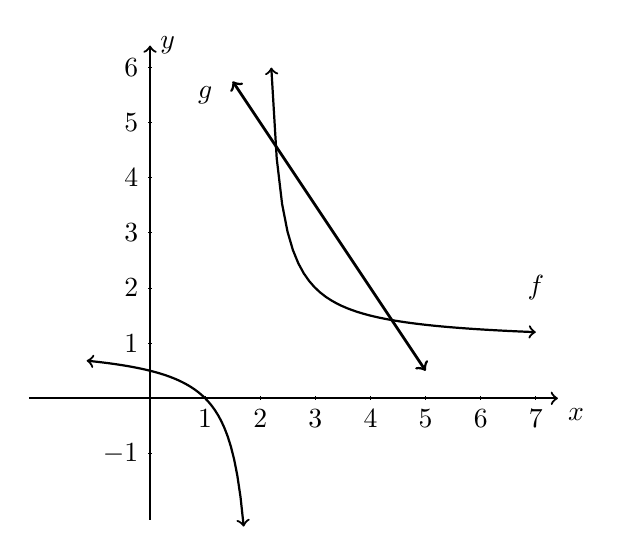
\begin{tikzpicture}[scale=0.7]
        %\draw [help lines] (-3,-3) grid (3,4);
        \draw [thick, ->] (-2.2,0) -- (7.4,0) node [below right] {$x$};
        \draw [thick, ->] (0,-2.2)--(0,6.4) node [right] {$y$};
        \foreach \x in {1,...,7} \draw (\x cm,1pt) -- (\x cm,-1pt) node[anchor=north] {$\x$};
        \foreach \y in {-1,1,2,...,6} \draw (1pt,\y cm) -- (-1pt,\y cm) node[left] {$\y$};
        %\clip (-2,-2) rectangle (6,7);
        \draw [<->,thick,samples=50,domain=2.2:7] plot(\x,{1/(\x-2)+1});
        \draw [<->,thick,samples=50,domain=-1.15:1.7] plot(\x,{1/(\x-2)+1});
        \draw [<->,line width=1.0pt,smooth,samples=20,domain=1.5:5] plot(\x,-1.5*\x+8);
        \node at (7,2){$f$};
        \node at (1,5.5){$g$};
      \end{tikzpicture}
    \end{flushright}
    \end{multicols}

\item Plot the function $h(x)=x^{3}+x^{2}-6x$, labeling the $x-$ and $y$-intercepts. Mark the local maximum and minimums as ordered pairs.
    \begin{center}
        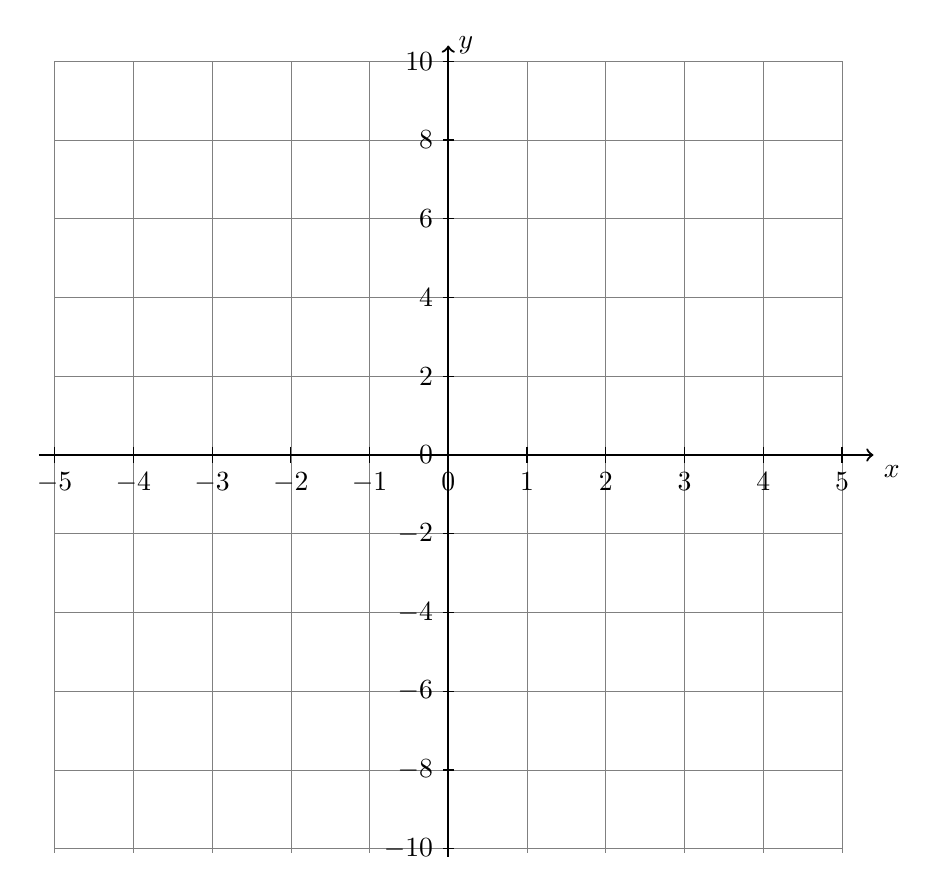
\begin{tikzpicture}[x=1cm, y=0.5cm]
            \draw [help lines] (-5,-10.1) grid (5,10);
            \draw [thick, ->] (-5.2,0) -- (5.4,0) node [below right] {$x$};
            \draw [thick, ->] (0,-10.2)--(0,10.4) node [right] {$y$};
            \foreach \x in {-5,...,5}
                \draw[shift={(\x,0)}] (0,3pt)--(0,-3pt) node[below] {$\x$};
            \foreach \y in {-10,-8,...,10}
                \draw[shift={(0,\y)}] (2pt,0pt)--(-2pt,0pt) node[left]  {$\y$};
            %\draw [<->,thick,smooth,domain=-3.5:2.5] plot(\x,{(\x)^3+(\x)^2-6*(\x)});
        \end{tikzpicture}
    \end{center}

\newpage
\item A cardboard box manufacturer is building boxes with length represented by $x+1$, width by $6-x$, and height by $x-2$. The volume of the box is modeled below.
    \begin{multicols}{2}
        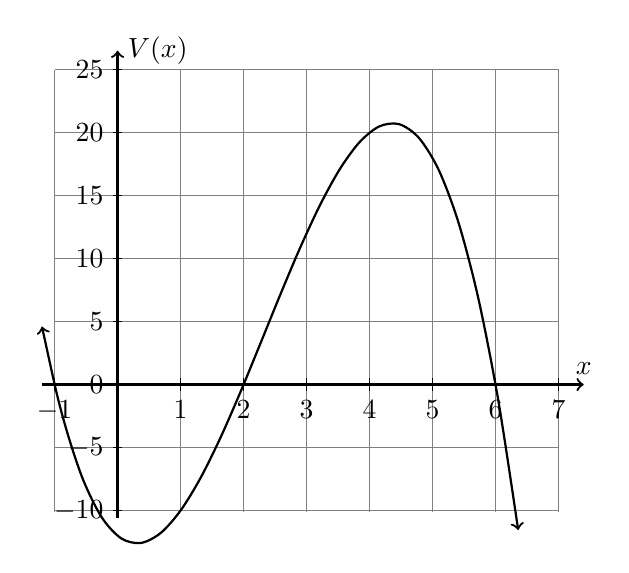
\begin{tikzpicture}[x=1cm, y=0.20cm, scale=0.8]
            \draw [help lines] (-1,-10.1) grid (7,25);
            \draw [thick, ->] (-1.2,0) -- (7.4,0) node [above] {$x$};
            \draw [thick, ->] (0,-10.6)--(0,26.5) node [right] {$V(x)$};
            \foreach \x in {-1,1,2,...,7}
                \draw[shift={(\x,0)}] (0,3pt)--(0,-3pt) node[below] {$\x$};
            \foreach \y in {-10,-5,...,25}
                \draw[shift={(0,\y)}] (2pt,0pt)--(-2pt,0pt) node[left]  {$\y$};
            \draw [<->,thick,smooth,domain=-1.2:6.36] plot(\x,{-(\x)^3+7*(\x)^2-4*(\x)-12});
        \end{tikzpicture}
    \begin{enumerate}[itemsep=0.75cm]
        \item Over what interval of positive $x$ values is the volume positive?
        \item Estimate the maximum possible volume of the box.
        \item Find the value of $x$ would maximize the volume of the box.
    \end{enumerate} 
\end{multicols}
%\vspace{0.5cm}

\item A function composed of four points $\{ (-2,1),(j,1),(3,4),(5,k) \}$ is plotted on the below.
    \begin{multicols}{2}
    \begin{enumerate}
      \item Write down $j$
      \item Write down $k$
      \item Write down the domain.\vspace{0.5cm}
      \item Add an ordered pair to the relation so that it would \emph{not} be a function.
    \end{enumerate}
      \begin{center}
      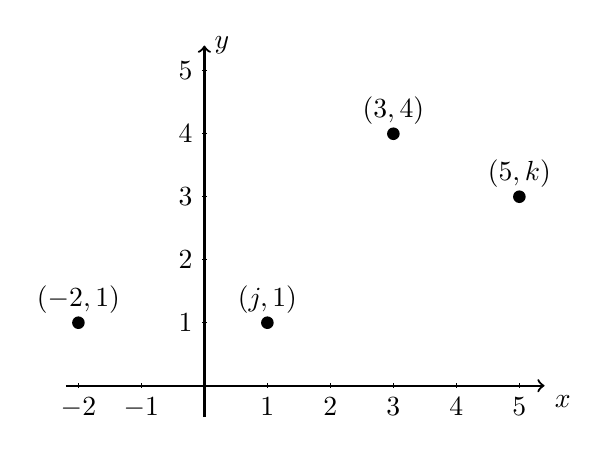
\begin{tikzpicture}[scale=0.8]
        %\draw [help lines] (-3,-2) grid (4,6);
        \draw [thick, ->] (-2.2,0) -- (5.4,0) node [below right] {$x$};
        \draw [thick, ->] (0,-0.5)--(0,5.4) node [right] {$y$};
        \foreach \x in {-2,-1,1,2,..., 5} \draw (\x cm,1pt) -- (\x cm,-1pt) node[anchor=north] {$\x$};
        \foreach \y in {1, 2, 3, 4, 5} \draw (1pt,\y cm) -- (-1pt,\y cm) node[anchor=east] {$\y$};
        %\draw [thick, <->] (-3.5,-1.5) -- (4.2,6.2);
        \fill (-2,1) circle[radius=0.1] node[above]{$(-2,1)$};
        \fill (1,1) circle[radius=0.1] node[above]{$(j,1)$};
        \fill (3,4) circle[radius=0.1] node[above]{$(3,4)$};
        \fill (5,3) circle[radius=0.1] node[above]{$(5,k)$};
      \end{tikzpicture}
      \end{center}
    \end{multicols}

\item A ski jump is modeled by the cubic function $h(x)=1.0+0.7x+0.8x^2-0.35x^{3}$ where $h$ is the height in meters above ground and $x$ is the horizontal distance (m).
\begin{multicols}{2}
    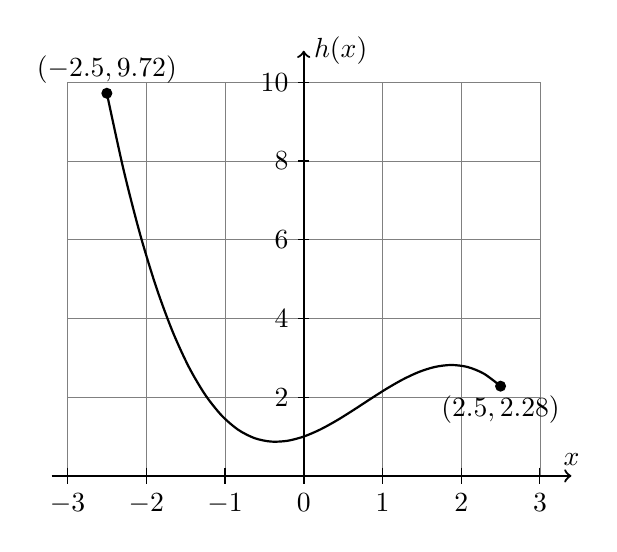
\begin{tikzpicture}[x=1cm, y=0.5cm, scale=1]
        \draw [help lines] (-3,0) grid (3,10);
        \draw [thick, ->] (-3.2,0) -- (3.4,0) node [above] {$x$};
        \draw [thick, ->] (0,-0.2)--(0,10.8) node [right] {$h(x)$};
        \foreach \x in {-3,...,3}
            \draw[shift={(\x,0)}] (0,3pt)--(0,-3pt) node[below] {$\x$};
        \foreach \y in {2,4,...,10}
            \draw[shift={(0,\y)}] (2pt,0pt)--(-2pt,0pt) node[left]  {$\y$};
        \draw [-,thick,smooth,domain=-2.5:2.5] plot(\x,{-0.35*(\x)^3+0.8*(\x)^2+0.7*(\x)+1});
        \fill (-2.5,9.72) ellipse(2pt and 2pt) node [above]{$(-2.5,9.72)$};
        \fill (2.5,2.28) ellipse(2pt and 2pt) node [below]{$(2.5,2.28)$};
    \end{tikzpicture}
    \begin{enumerate}[itemsep=0.5cm]
        \item The two ends of the ramp are marked as ordered pairs. How wide is the ramp in meters?
        \item What is the total vertical descent from the top of the ramp to its lowest point? \vspace{1cm}\\ \, %answer 8.85m
    \end{enumerate} 
    \end{multicols}

\newpage
\item Shown in the plot below is the function $f(x)=x^3-x^2-9x+9$.
    \begin{enumerate}
        \item Write down the value of $f(0)$. On the graph, mark the point for $f(0)$ with a star.\vspace{0.75cm}
        \item Write down the solutions to $f(x)=0$. Mark them with ``X'' marks on the graph.\vspace{0.75cm}
        \item Mark the portion of the function that is \emph{decreasing} with a squiggly line.
    \end{enumerate}
    \begin{center}
        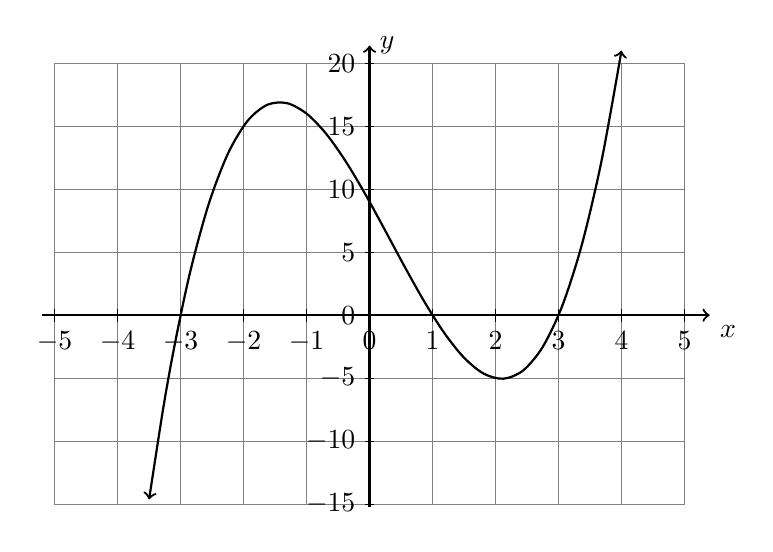
\begin{tikzpicture}[x=1cm, y=0.20cm, scale=0.8]
            \draw [help lines] (-5,-15.1) grid (5,20);
            \draw [thick, ->] (-5.2,0) -- (5.4,0) node [below right] {$x$};
            \draw [thick, ->] (0,-15.2)--(0,21.4) node [right] {$y$};
            \foreach \x in {-5,...,5}
                \draw[shift={(\x,0)}] (0,3pt)--(0,-3pt) node[below] {$\x$};
            \foreach \y in {-15,-10,...,20}
                \draw[shift={(0,\y)}] (2pt,0pt)--(-2pt,0pt) node[left]  {$\y$};
            \draw [<->,thick,smooth,domain=-3.5:4] plot(\x,{(\x)^3-(\x)^2-9*(\x)+9});
        \end{tikzpicture}
    \end{center}

\item The function $f(x)=ax^2+bx+c$ is graphed below over its domain, $p\leq x < q$.
    \begin{multicols}{2}
    \begin{enumerate}
      \item Write down the value of $c$.
      \item Write down $f(-2)$.
      \item Find $x$ such that $f(x)=6$.
      \item Write down the values of $p$, $q$.
      \item Write down the range of $f$. \vspace{1cm}
    \end{enumerate}
      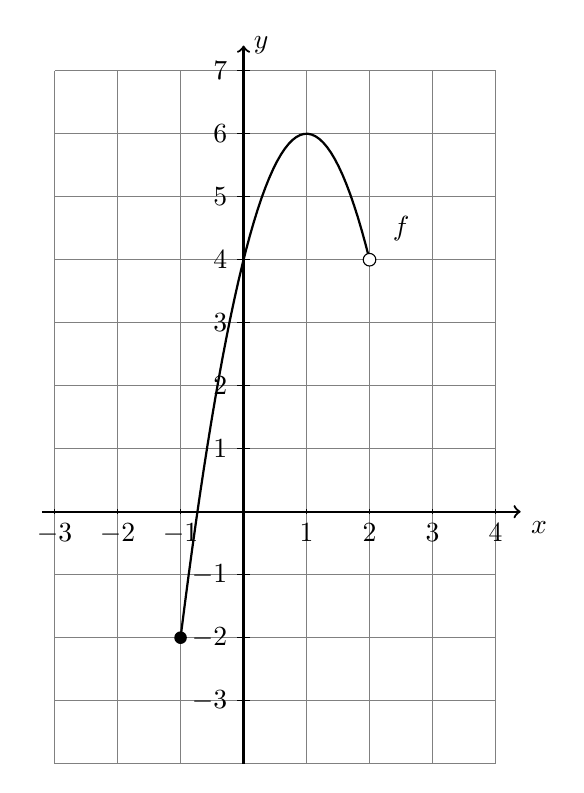
\begin{tikzpicture}[scale=0.8]
        \draw [help lines] (-3,-4) grid (4,7);
        \draw [thick, ->] (-3.2,0) -- (4.4,0) node [below right] {$x$};
        \draw [thick, ->] (0,-4)--(0,7.4) node [right] {$y$};
        \foreach \x in {-3,-2,-1,1,2, ..., 4} \draw (\x cm,1pt) -- (\x cm,-1pt) node[below] {$\x$};
        \foreach \y in {-3,-2,-1,1,2,...,7} \draw (3pt,\y cm) -- (-3pt,\y cm) node[left] {$\y$};
        \draw [thick,samples=50,domain=-1:2] plot(\x,-2*\x*\x+4*\x+4);
        \fill (-1,-2) circle[radius=0.1];
        \node at (2.5,4.5){$f$};
        \fill [white] (2,4) circle[radius=0.1];
        \draw (2,4) circle[radius=0.1];
      \end{tikzpicture}
    \end{multicols}
    \vspace{0.5cm}

\newpage    
\item A rational function of the form $\displaystyle f(x)=\frac{1}{x-p}+q$ is shown on the grid below. 
    \begin{multicols}{2}
        \begin{enumerate}[itemsep=0.7cm]
            \item Write down the equation of the horizontal asymptote.
            \item  Write down the equation of the vertical asymptote.
            \item Hence, write down $p$ and $q$.
            \item Find $f(0)$.
            \item Solve for $x$ such that $f(x)=0$. \vspace{1cm} \\ \,
        \end{enumerate}
        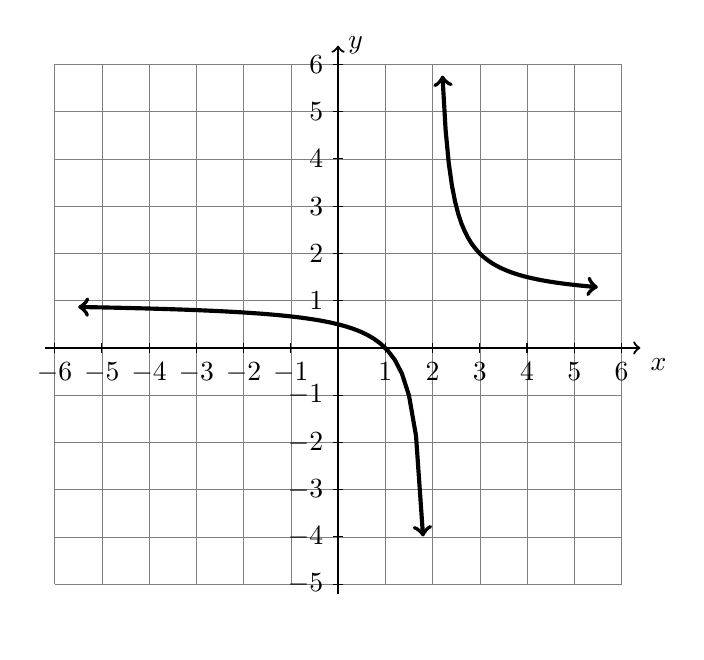
\begin{tikzpicture}[scale=0.6]
        \draw [help lines] (-6,-5) grid (6,6);
        \draw [thick, ->] (-6.2,0) -- (6.4,0) node [below right] {$x$};
        \draw [thick, ->] (0,-5.2)--(0,6.4) node [right] {$y$};
        \foreach \x in {-6,...,-3,-2,-1,1,2,...,6} \draw (\x cm,3pt) -- (\x cm,-3pt) node[below] {$\x$};
        \foreach \y in {-5,...,-3,-2,-1,1,2,...,6} \draw (3pt,\y cm) -- (-3pt,\y cm) node[left] {$\y$};
        \clip (-6,-6) rectangle (6,6);
        \draw [<->,line width=1.5pt,samples=50,domain=-5.5:1.8] plot(\x,{1/(\x-2)+1});
        \draw [<->,line width=1.5pt,samples=50,domain=2.21:5.5] plot(\x,{1/(\x-2)+1});
        \end{tikzpicture}
    \end{multicols}

\item The temperature ($C^\circ$) over a 24 hour day starting at midnight is modeled by the function $f\left(t\right)=-0.0063t^{3}+0.12t^{2}+0.38t+9$.
    \begin{enumerate}[itemsep=1cm]
        \item Write down the temperature at midnight, when $t=0$.
        \item Over what interval is the temperature increasing?
        \item Find the maximum temperature during the day.  \vspace{1cm}
    \end{enumerate}
    \begin{center}
    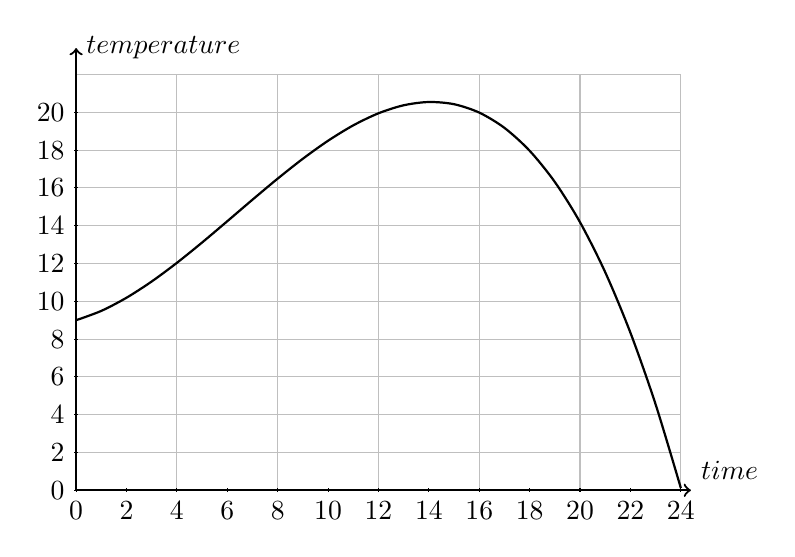
\begin{tikzpicture}[xscale=0.4, yscale=0.3, scale=0.8]
        \draw [thin, color=lightgray, xstep=4.0cm,ystep=2.0cm] (0,0) grid (24,22);
        \foreach \x in {0,2,...,24}
        \draw (\x cm,3pt) -- (\x cm,-3pt) node[below] {$\x$};
        \foreach \y in {0,2,...,20}
        \draw[shift={(0,\y)},color=black] (2pt,0pt) -- (-2pt,0pt) node[left]{$\y$};
        \draw [thick, ->] (0,0) -- (+24.4,0) node [above right]{$time$};
        \draw [thick, ->] (0,0) -- (0,23.4) node [right]{$temperature$};
        \draw [thick, smooth,domain=0.:24] plot(\x,-0.0063*\x*\x*\x+0.12*\x*\x+0.38*\x+9);
    \end{tikzpicture}
    \end{center}

\end{enumerate}
\end{document}



